% Compile with: pdflatex intro.tex
\documentclass[aspectratio=169]{beamer}

\usetheme{Madrid}
\usecolortheme{seahorse}
\setbeamertemplate{navigation symbols}{}
\setbeamertemplate{footline}[frame number]
\setbeamerfont{frametitle}{size=\Large, series=\bfseries}
\setbeamercolor{block title}{bg=blue!15, fg=black}
\setbeamercolor{block body}{bg=blue!5}

\usepackage[utf8]{inputenc}
\usepackage[T1]{fontenc}
\usepackage{lmodern}
\usepackage{tikz}
\usetikzlibrary{positioning, arrows.meta, shapes.symbols, shapes.geometric}

\tikzset{
  bblock/.style  = {draw, rounded corners, minimum width=2.3cm, minimum height=1.2cm, align=center, font=\small},
  stepbox/.style = {draw, rounded corners, minimum width=3.8cm, minimum height=2.2cm, text width=3.4cm, align=center, fill=blue!10},
  concept/.style = {draw, rounded corners, minimum width=3.4cm, minimum height=2cm, text width=3cm, align=center, fill=blue!8},
  arrow/.style   = {-Stealth, very thick}
}

\title{Blockchain 101}
\subtitle{Your first smart contract}
\author{UMons}
\date{}

\begin{document}

% =====================================================================
\begin{frame}
  \titlepage
\end{frame}

% =====================================================================
\begin{frame}{What is a blockchain?}
\centering
\vspace{0.4em}

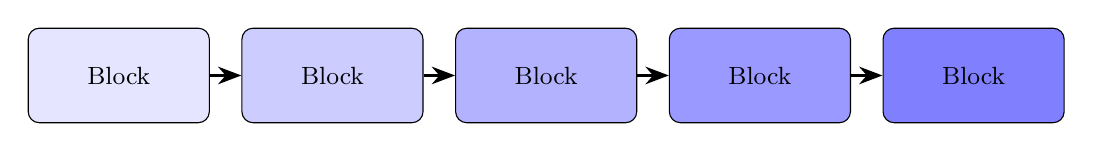
\begin{tikzpicture}
  \node[bblock, fill=blue!10]                   (b1) {Block};
  \node[bblock, fill=blue!20, right=0.4cm of b1] (b2) {Block};
  \node[bblock, fill=blue!30, right=0.4cm of b2] (b3) {Block};
  \node[bblock, fill=blue!40, right=0.4cm of b3] (b4) {Block};
  \node[bblock, fill=blue!50, right=0.4cm of b4] (b5) {Block};
  \draw[arrow] (b1) -- (b2);
  \draw[arrow] (b2) -- (b3);
  \draw[arrow] (b3) -- (b4);
  \draw[arrow] (b4) -- (b5);
\end{tikzpicture}

\vspace{1.4em}

{\Large A \textbf{public database} that anyone can read.}\\[0.4em]
{\Large Append-only. Signed. Unstoppable.}

\vspace{1.2em}
\small\itshape Smart contracts = programs that live on it.
\end{frame}

% =====================================================================
\begin{frame}{The 4 words you need}
\vspace{0.6em}
\centering

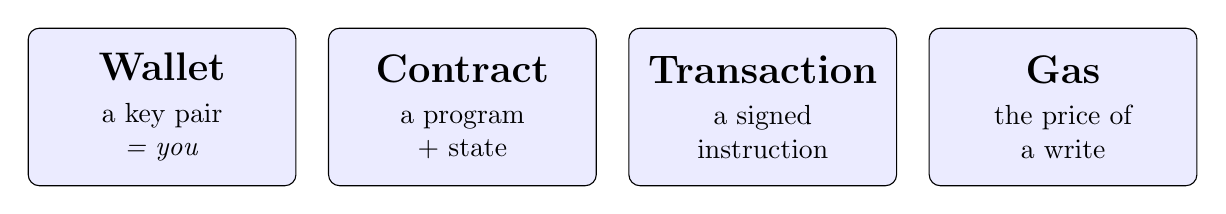
\begin{tikzpicture}
  \node[concept] (w) {{\Large\bfseries Wallet}\\[0.3em] a key pair\\ \textit{= you}};
  \node[concept, right=0.4cm of w] (c) {{\Large\bfseries Contract}\\[0.3em] a program\\ + state};
  \node[concept, right=0.4cm of c] (t) {{\Large\bfseries Transaction}\\[0.3em] a signed\\ instruction};
  \node[concept, right=0.4cm of t] (g) {{\Large\bfseries Gas}\\[0.3em] the price of\\ a write};
\end{tikzpicture}

\vspace{1.6em}
{\large Reading is \textbf{free}.\quad Writing costs \textbf{gas}.}

\end{frame}

% =====================================================================
\begin{frame}{Life of a transaction}
\vspace{0.4em}
\centering

\resizebox{\textwidth}{!}{%
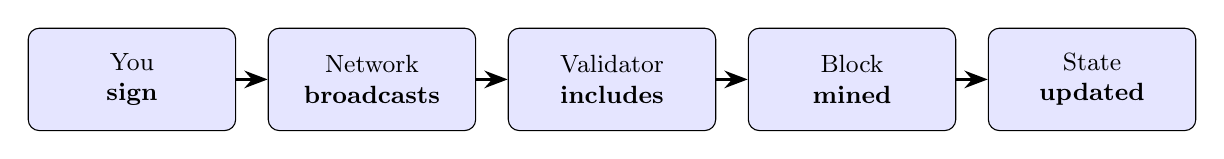
\begin{tikzpicture}[
  node distance=0.4cm,
  bx/.style={draw, rounded corners, minimum height=1.3cm, text width=2.4cm, align=center, fill=blue!10, font=\small}
]
  \node[bx] (a) {You\\ \textbf{sign}};
  \node[bx, right=of a] (b) {Network\\ \textbf{broadcasts}};
  \node[bx, right=of b] (c) {Validator\\ \textbf{includes}};
  \node[bx, right=of c] (d) {Block\\ \textbf{mined}};
  \node[bx, right=of d] (e) {State\\ \textbf{updated}};

  \draw[arrow] (a) -- (b);
  \draw[arrow] (b) -- (c);
  \draw[arrow] (c) -- (d);
  \draw[arrow] (d) -- (e);
\end{tikzpicture}%
}

\vspace{1.6em}
{\large Takes a few seconds on Arbitrum. Costs a fraction of a cent.}\\[0.6em]
\small\itshape Once mined, the change is \textbf{permanent} and visible to the whole world.

\end{frame}

% =====================================================================
\begin{frame}{What we will build}

\vspace{0.3em}
\centering
{\Large A contract called \texttt{SimpleStorage}}

\vspace{0.8em}

\begin{columns}[T,onlytextwidth]
\begin{column}{0.52\textwidth}
\centering
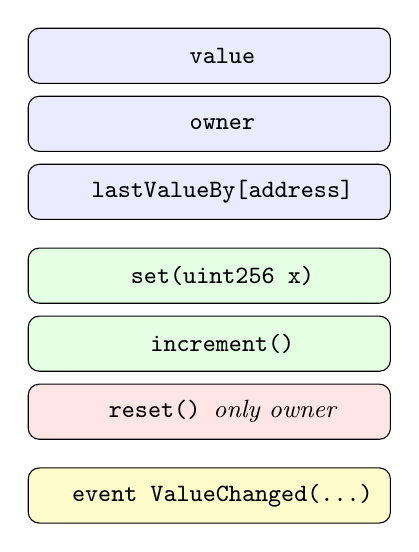
\begin{tikzpicture}[
  fn/.style={draw, rounded corners, minimum width=4.6cm, minimum height=0.7cm, align=left, fill=blue!8, font=\small\ttfamily}
]
  \node[fn]                       (f1) {\quad value};
  \node[fn, below=0.15cm of f1]   (f2) {\quad owner};
  \node[fn, below=0.15cm of f2]   (f3) {\quad lastValueBy[address]};
  \node[fn, below=0.35cm of f3, fill=green!10] (f4) {\quad set(uint256 x)};
  \node[fn, below=0.15cm of f4, fill=green!10] (f5) {\quad increment()};
  \node[fn, below=0.15cm of f5, fill=red!10]   (f6) {\quad reset()  \rmfamily\itshape only owner};
  \node[fn, below=0.35cm of f6, fill=yellow!20] (f7) {\quad event ValueChanged(...)};
\end{tikzpicture}
\end{column}

\begin{column}{0.48\textwidth}
\vspace{0.6em}
\begin{itemize}
  \item Stores a number\vspace{0.15em}
  \item Anyone can change it\vspace{0.15em}
  \item Tracks who wrote what\vspace{0.15em}
  \item Only the deployer can \texttt{reset}
\end{itemize}

\vspace{0.6em}
\small\textbf{What's an event?}\\
A log line the contract emits.\\
It does \emph{not} change state, but it is \textbf{saved on-chain} and anyone can subscribe to it --- great for dApps that want to react in real time.
\end{column}
\end{columns}

\end{frame}

% =====================================================================
\begin{frame}{Today's goal}
\vspace{1em}
\centering

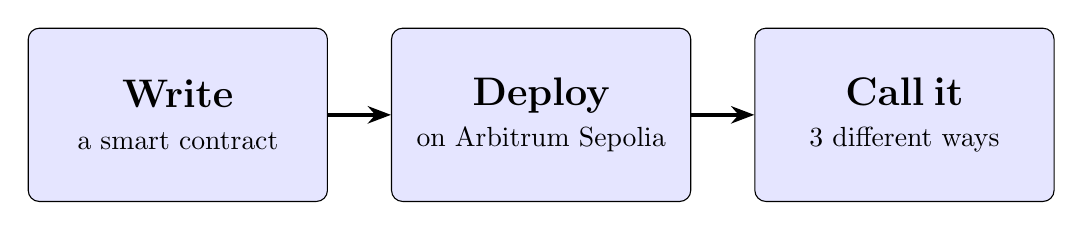
\begin{tikzpicture}
  \node[stepbox] (write)  {{\Large\bfseries Write}\\[0.3em] a smart contract};
  \node[stepbox, right=0.8cm of write]  (deploy) {{\Large\bfseries Deploy}\\[0.3em] on Arbitrum Sepolia};
  \node[stepbox, right=0.8cm of deploy] (call)   {{\Large\bfseries Call it}\\[0.3em] 3 different ways};
  \draw[arrow] (write)  -- (deploy);
  \draw[arrow] (deploy) -- (call);
\end{tikzpicture}

\vspace{2em}
{\Large Your code, live on the public Internet.}
\end{frame}

% =====================================================================
\begin{frame}{3 ways to call your contract}
\vspace{0.3em}
\centering

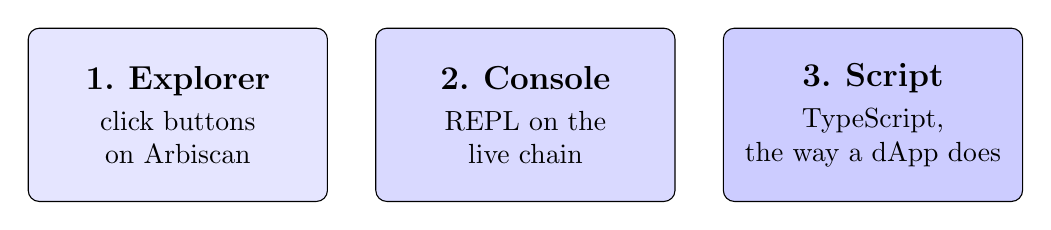
\begin{tikzpicture}
  \node[stepbox, fill=blue!10]                            (w1) {{\large\bfseries 1. Explorer}\\[0.3em] click buttons\\ on Arbiscan};
  \node[stepbox, fill=blue!15, right=0.6cm of w1]         (w2) {{\large\bfseries 2. Console}\\[0.3em] REPL on the\\ live chain};
  \node[stepbox, fill=blue!20, right=0.6cm of w2]         (w3) {{\large\bfseries 3. Script}\\[0.3em] TypeScript,\\ the way a dApp does};
\end{tikzpicture}

\vspace{1.4em}
{\large Same contract. Three angles to understand it.}\\[0.5em]
\small\itshape Read = free.\quad Write = signed transaction + gas.

\end{frame}

% =====================================================================
\begin{frame}{Resources}
\vspace{0.6em}
\centering

\begin{tabular}{rl}
  \textbf{Docs}     & \texttt{tanguyvans.github.io/blockchain-101} \\[0.3em]
  \textbf{Repo}     & \texttt{github.com/tanguyvans/blockchain-101} \\[0.3em]
  \textbf{Network}  & Arbitrum Sepolia (chain id 421614) \\[0.3em]
  \textbf{Explorer} & \texttt{sepolia.arbiscan.io} \\[0.3em]
  \textbf{Faucet}   & \texttt{faucet.quicknode.com/arbitrum/sepolia} \\
\end{tabular}

\vspace{1em}
\centering
\fbox{\parbox{0.85\textwidth}{\centering
\small\textbf{Need test ETH?} Email me your public address at\\
\texttt{tanguy.vansnick@umons.ac.be} and I will send you faucet funds.
}}

\vspace{1em}
{\Huge Let's build.}

\end{frame}

\end{document}
